\documentclass[border=2pt]{standalone}
\usepackage{amsmath}
\usepackage{tikz}
\usetikzlibrary{arrows.meta,shapes.symbols}
\begin{document}
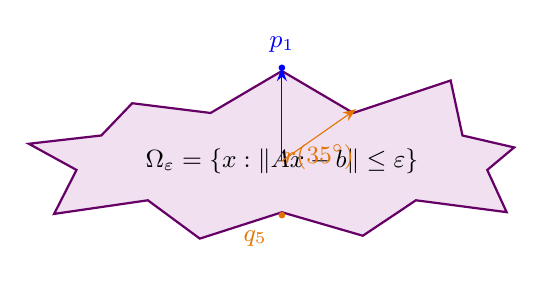
\begin{tikzpicture}[>=Stealth,every node/.style={font=\small}]
  \node[starburst,starburst points=9,starburst point height=7mm,
    random starburst=314,shape border rotate=18,
    minimum width=42mm,minimum height=27mm,inner sep=4pt,outer sep=1pt,
    draw=violet!80!black,fill=violet!12,thick] (set)
    {$\Omega_{\varepsilon}=\{x:\lVert Ax-b\rVert\leq\varepsilon\}$};
  \fill[blue] (set.outer point 1) circle (1.2pt) node[above=2pt] {$p_1$};
  \fill[orange!90!black] (set.inner point 5) circle (1.2pt)
    node[below left=2pt] {$q_5$};
  \draw[->,blue] (set.center) -- (set.outer point 1);
  \draw[->,orange!90!black] (set.center) -- (set.35)
    node[midway,below] {$r(35^\circ)$};
\end{tikzpicture}
\end{document}
